% ============================================================================
% SIH 26171 - Architecture diagram (print/high-res PDF)
% Compile: pdflatex architecture.tex
% ============================================================================
\documentclass[border=10pt]{standalone}
\usepackage[T1]{fontenc}
\usepackage[utf8]{inputenc}
\usepackage{lmodern}
\usepackage{xcolor}
\usepackage{tikz}
\usetikzlibrary{arrows.meta}

\definecolor{primary}{RGB}{40,53,147}
\definecolor{secondary}{RGB}{13,110,253}
\definecolor{accent}{RGB}{182,40,53}
\definecolor{good}{RGB}{21,128,61}

\begin{document}

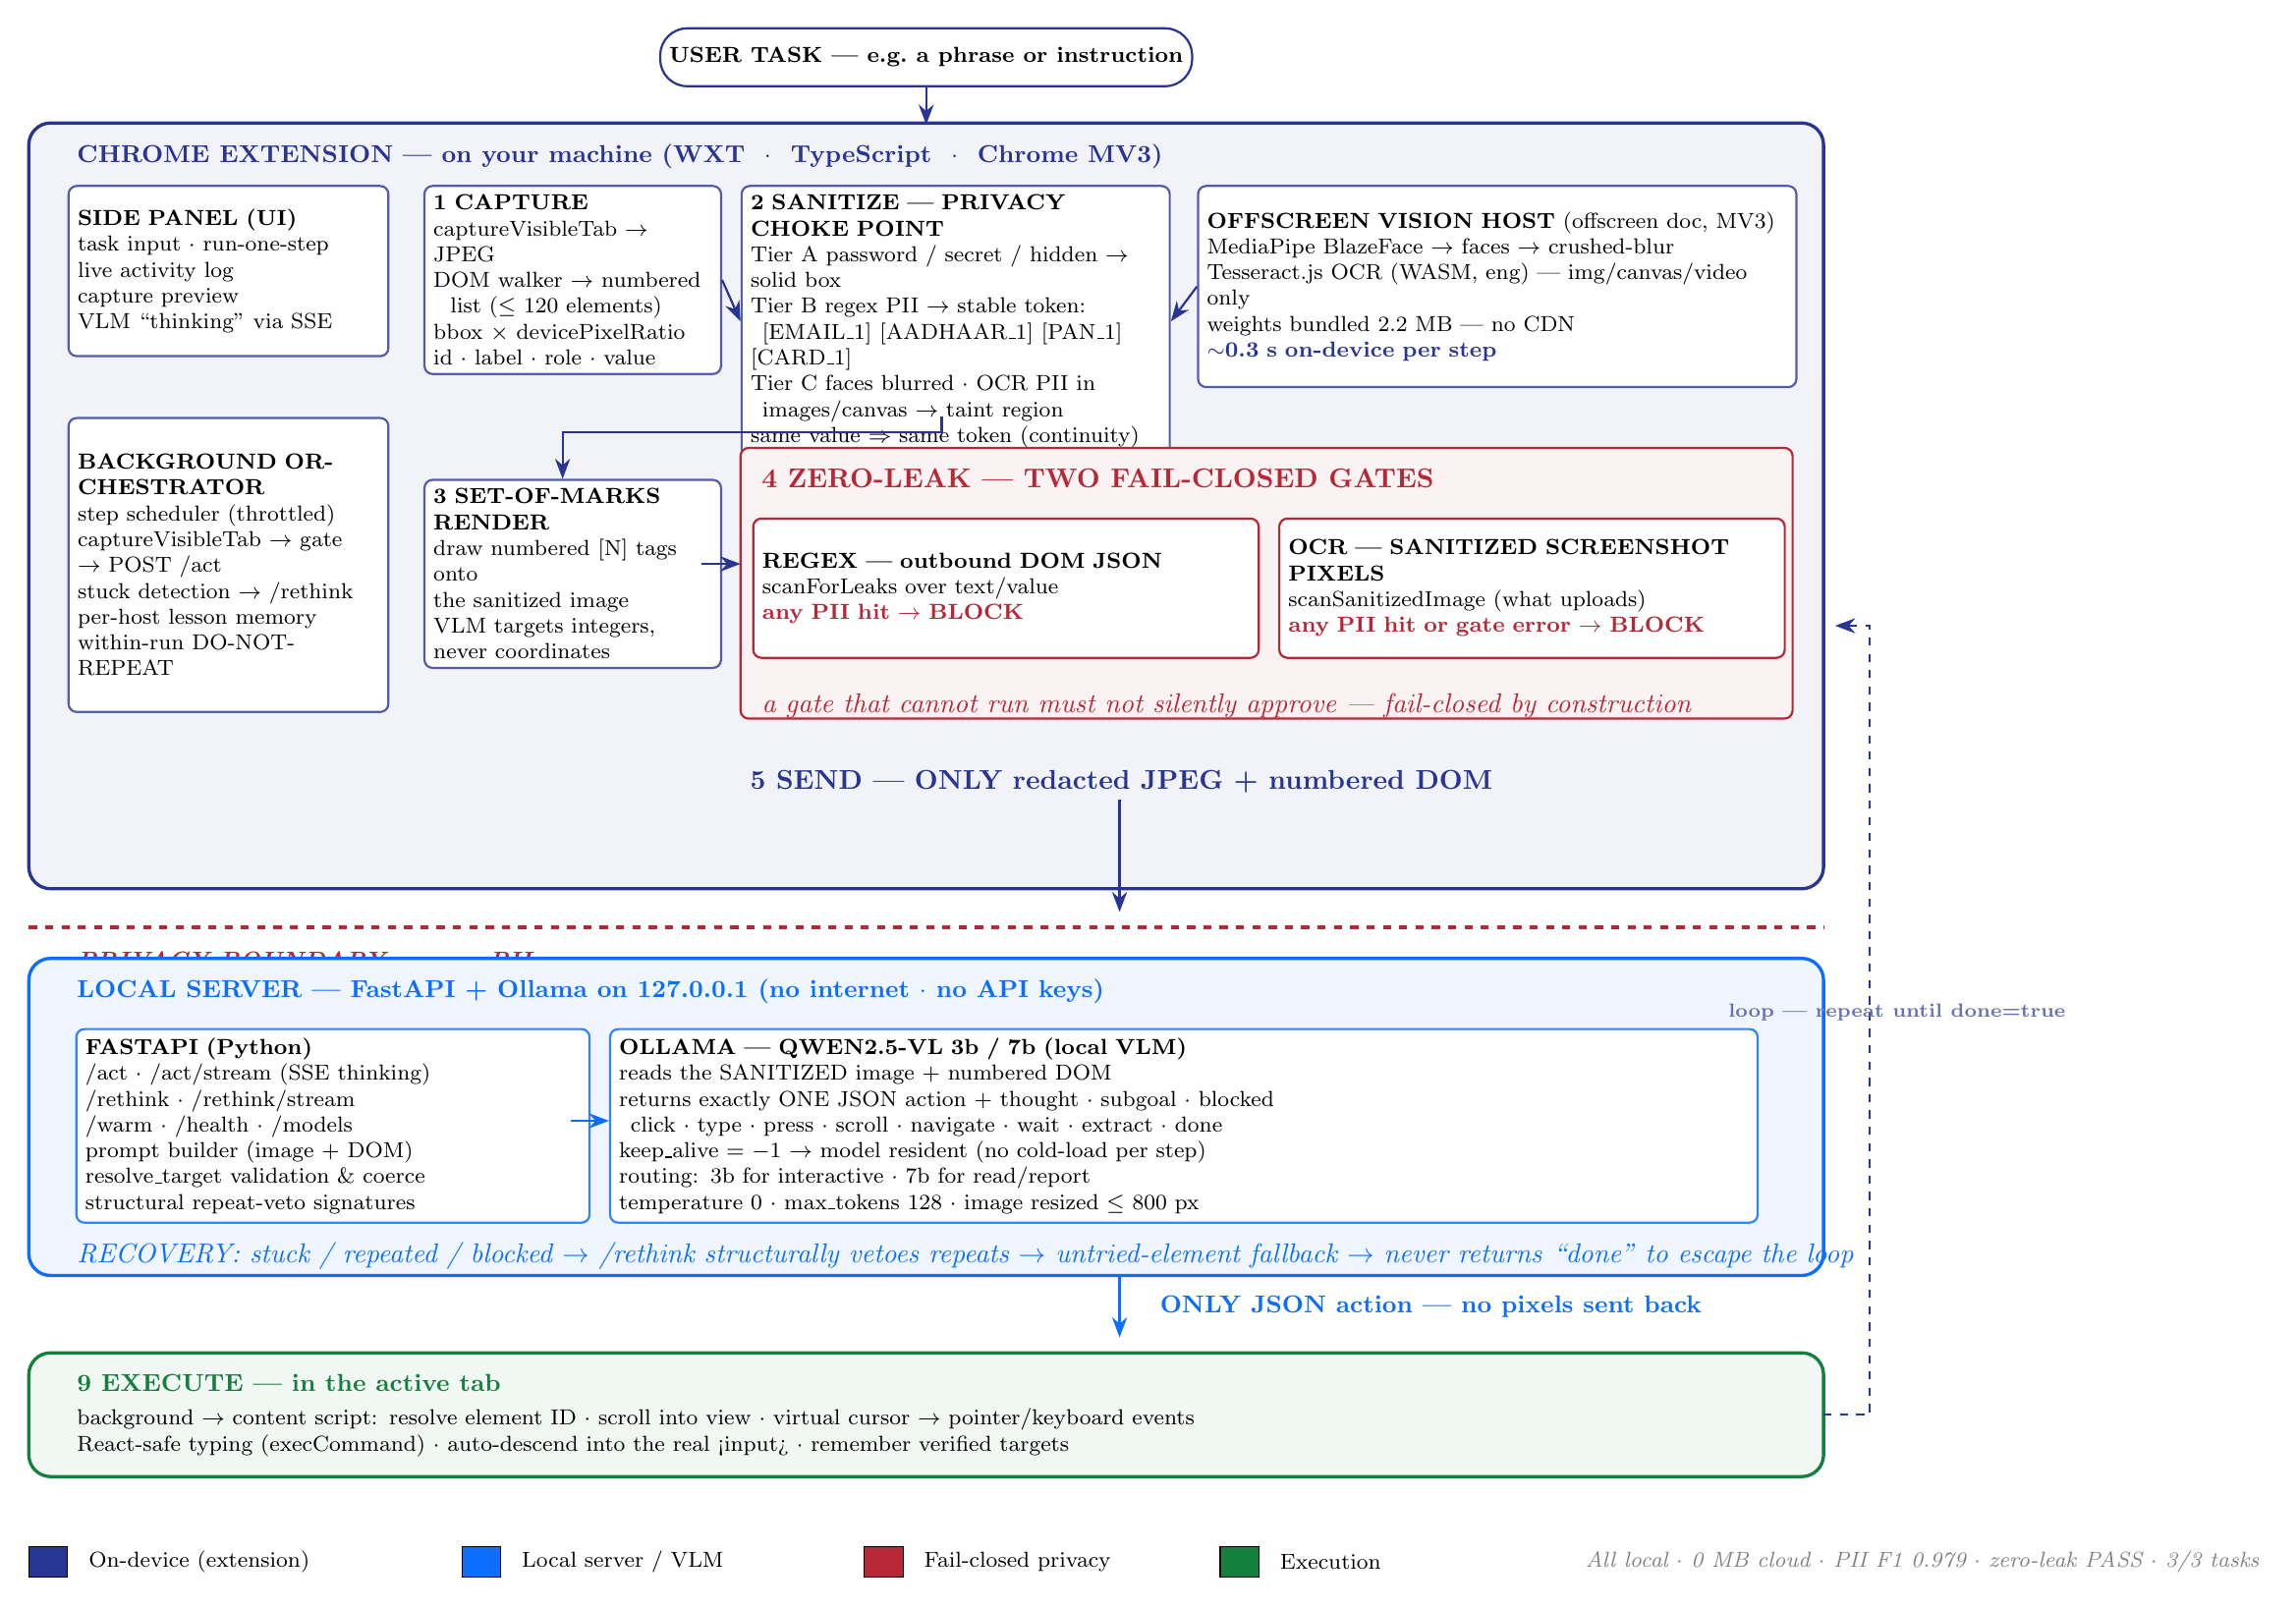
\begin{tikzpicture}[
  x=1cm, y=-1cm,        % positive y goes DOWN the page (natural reading order)
  font=\footnotesize,
  bandext/.style={draw=primary, very thick, rounded corners=8pt, fill=primary!6},
  bandsrv/.style={draw=secondary, very thick, rounded corners=8pt, fill=secondary!6},
  bandexe/.style={draw=good, very thick, rounded corners=8pt, fill=good!6},
  box/.style={draw=primary!80, thick, rounded corners=3pt, fill=white},
  boxb/.style={draw=secondary!85, thick, rounded corners=3pt, fill=white},
  subr/.style={draw=accent, thick, rounded corners=3pt, fill=white},
  pill/.style={draw=primary, thick, rounded corners=10pt, fill=white},
  main/.style={-{Stealth[length=2.6mm]}, thick, color=primary},
  arb/.style={-{Stealth[length=2.6mm]}, thick, color=secondary},
]

% ============================ USER TASK ============================
\node[pill, anchor=center, minimum width=6cm, minimum height=0.75cm] (task) at (12,0.85)
  {\bfseries USER TASK --- e.g.\ a phrase or instruction};
\draw[main] (12,1.22) -- (12,1.72);

% ============================ EXTENSION BAND ============================
\draw[bandext] (0.4,1.7) rectangle (23.6,11.6);
\node[anchor=north west, font=\bfseries\small, text=primary] at (0.9,1.85)
  {CHROME EXTENSION --- on your machine (WXT ~$\cdot$~ TypeScript ~$\cdot$~ Chrome MV3)};

% -- side panel --
\node[box, anchor=north west, text width=3.9cm, align=left, minimum height=2.2cm] (panel) at (0.9,2.5)
  {\textbf{SIDE PANEL (UI)}\\
   task input $\cdot$ run-one-step\\
   live activity log\\
   capture preview\\
   VLM ``thinking'' via SSE};

% -- background --
\node[box, anchor=north west, text width=3.9cm, align=left, minimum height=3.8cm] (bg) at (0.9,5.5)
  {\textbf{BACKGROUND ORCHESTRATOR}\\
   step scheduler (throttled)\\
   captureVisibleTab $\rightarrow$ gate\\
   $\rightarrow$ POST /act\\
   stuck detection $\rightarrow$ /rethink\\
   per-host lesson memory\\
   within-run DO-NOT-REPEAT};

% -- 1 capture --
\node[box, anchor=north west, text width=3.6cm, align=left, minimum height=2.1cm] (cap) at (5.5,2.5)
  {\textbf{1 CAPTURE}\\
   captureVisibleTab $\rightarrow$ JPEG\\
   DOM walker $\rightarrow$ numbered\\
   \hspace*{0.4em} list ($\leq$ 120 elements)\\
   bbox $\times$ devicePixelRatio\\
   id $\cdot$ label $\cdot$ role $\cdot$ value};

% -- 2 sanitize --
\node[box, anchor=north west, text width=5.3cm, align=left, minimum height=3.0cm] (san) at (9.6,2.5)
  {\textbf{2 SANITIZE --- PRIVACY CHOKE POINT}\\
   Tier A\ password / secret / hidden $\rightarrow$ solid box\\
   Tier B\ regex PII $\rightarrow$ stable token:\\
   \hspace*{0.5em}[EMAIL\_1] [AADHAAR\_1] [PAN\_1] [CARD\_1]\\
   Tier C\ faces blurred $\cdot$ OCR PII in\\
   \hspace*{0.5em}images/canvas $\rightarrow$ taint region\\
   same value $\Rightarrow$ same token (continuity)};

% -- vision host --
\node[box, anchor=north west, text width=7.5cm, align=left, minimum height=2.6cm] (vis) at (15.5,2.5)
  {\textbf{OFFSCREEN VISION HOST}~(offscreen doc, MV3)\\
   MediaPipe BlazeFace $\rightarrow$ faces $\rightarrow$ crushed-blur\\
   Tesseract.js OCR (WASM, eng) --- img/canvas/video only\\
   weights bundled 2.2 MB --- no CDN\\
   \textbf{\textcolor{primary}{$\sim$0.3 s on-device per step}}};

\draw[main] (cap.east) -- (san.west);
\draw[main] (vis.west) -- (san.east);

% -- 3 set-of-marks --
\node[box, anchor=north west, text width=3.6cm, align=left, minimum height=2.2cm] (som) at (5.5,6.3)
  {\textbf{3 SET-OF-MARKS RENDER}\\
   draw numbered [N] tags onto\\
   the sanitized image\\
   VLM targets integers,\\
   never coordinates};

% sanitize -> set-of-marks (elbow)
\draw[main] (12.2,5.5) -- (12.2,5.7) -- (7.3,5.7) -- (7.3,6.3);

% -- 4 zero-leak (manual layout) --
\draw[fill=accent!6, draw=accent, thick, rounded corners=3pt] (9.6,5.9) rectangle (23.2,9.4);
\node[anchor=north west, font=\bfseries, text=accent] at (9.75,6.05)
  {4 ZERO-LEAK --- TWO FAIL-CLOSED GATES};
\node[subr, anchor=north west, text width=6.3cm, align=left, minimum height=1.8cm] at (9.75,6.8)
  {\textbf{REGEX --- outbound DOM JSON}\\
   scanForLeaks over text/value\\
   \textcolor{accent}{\textbf{any PII hit $\rightarrow$ BLOCK}}};
\node[subr, anchor=north west, text width=6.3cm, align=left, minimum height=1.8cm] at (16.55,6.8)
  {\textbf{OCR --- SANITIZED SCREENSHOT PIXELS}\\
   scanSanitizedImage (what uploads)\\
   \textcolor{accent}{\textbf{any PII hit or gate error $\rightarrow$ BLOCK}}};
\node[anchor=north west, font=\itshape, text=accent] at (9.75,8.95)
  {a gate that cannot run must not silently approve --- fail-closed by construction};

% set-of-marks -> zero-leak
\draw[main] (9.1,7.4) -- (9.6,7.4);

% -- 5 send --
\node[anchor=north west, font=\bfseries, text=primary] at (9.6,9.95)
  {5 SEND --- ONLY redacted JPEG + numbered DOM};
\draw[main] (14.5,10.45) -- (14.5,11.9);

% -- privacy boundary --
\draw[accent, dashed, very thick] (0.4,12.1) -- (23.6,12.1);
\node[anchor=north west, font=\bfseries\itshape\small, text=accent] at (0.9,12.3)
  {PRIVACY BOUNDARY --- raw PII never crosses};

% ============================ SERVER BAND ============================
\draw[bandsrv] (0.4,12.5) rectangle (23.6,16.6);
\node[anchor=north west, font=\bfseries\small, text=secondary] at (0.9,12.65)
  {LOCAL SERVER --- FastAPI + Ollama on 127.0.0.1 (no internet $\cdot$ no API keys)};

\node[boxb, anchor=north west, text width=6.4cm, align=left, minimum height=2.4cm] (fapi) at (1.0,13.4)
  {\textbf{FASTAPI (Python)}\\
   /act $\cdot$ /act/stream (SSE thinking)\\
   /rethink $\cdot$ /rethink/stream\\
   /warm $\cdot$ /health $\cdot$ /models\\
   prompt builder (image + DOM)\\
   resolve\_target validation \& coerce\\
   structural repeat-veto signatures};
\node[boxb, anchor=north west, text width=14.6cm, align=left, minimum height=2.4cm] (oll) at (7.9,13.4)
  {\textbf{OLLAMA --- QWEN2.5-VL 3b / 7b (local VLM)}\\
   reads the SANITIZED image + numbered DOM\\
   returns exactly ONE JSON action + thought $\cdot$ subgoal $\cdot$ blocked\\
   \hspace*{0.5em}click $\cdot$ type $\cdot$ press $\cdot$ scroll $\cdot$ navigate $\cdot$ wait $\cdot$ extract $\cdot$ done\\
   keep\_alive = $-1$ $\rightarrow$ model resident (no cold-load per step)\\
   routing: 3b for interactive $\cdot$ 7b for read/report\\
   temperature 0 $\cdot$ max\_tokens 128 $\cdot$ image resized $\leq$ 800 px};
\draw[arb] (7.4,14.6) -- (7.9,14.6);

\node[anchor=north west, font=\itshape, text=secondary] at (0.9,16.05)
  {RECOVERY: stuck / repeated / blocked $\rightarrow$ /rethink structurally vetoes repeats $\rightarrow$ untried-element fallback $\rightarrow$ never returns ``done'' to escape the loop};

% ============================ JSON RETURN ============================
\draw[arb] (14.5,16.6) -- (14.5,17.4);
\node[anchor=west, font=\bfseries\small, text=secondary] at (14.9,17.0)
  {ONLY JSON action --- no pixels sent back};

% ============================ EXECUTE ============================
\draw[bandexe] (0.4,17.6) rectangle (23.6,19.2);
\node[anchor=north west, font=\bfseries\small, text=good] (exe) at (0.9,17.75)
  {9 EXECUTE --- in the active tab};
\node[anchor=north west, text width=22cm, align=left] at (0.9,18.2)
  {background $\rightarrow$ content script: resolve element ID $\cdot$ scroll into view $\cdot$ virtual cursor $\rightarrow$ pointer/keyboard events\\
   React-safe typing (execCommand) $\cdot$ auto-descend into the real <input> $\cdot$ remember verified targets};

% ============================ LOOP BACK ============================
\draw[main, dashed] (23.6,18.4) -- (24.2,18.4) -- (24.2,8.2) -- (23.75,8.2);
\node[text=primary!70, font=\scriptsize\bfseries] at (24.55,13.2) {loop --- repeat until done=true};

% ============================ LEGEND ============================
\draw[fill=primary]  (0.4,20.1) rectangle (0.9,20.5);
\node[anchor=west] at (1.05,20.3) {On-device (extension)};
\draw[fill=secondary] (6.0,20.1) rectangle (6.5,20.5);
\node[anchor=west] at (6.65,20.3) {Local server / VLM};
\draw[fill=accent]    (11.2,20.1) rectangle (11.7,20.5);
\node[anchor=west] at (11.85,20.3) {Fail-closed privacy};
\draw[fill=good]      (15.8,20.1) rectangle (16.3,20.5);
\node[anchor=west] at (16.45,20.3) {Execution};
\node[anchor=west, text=black!50, font=\itshape\footnotesize] at (20.4,20.3)
  {All local $\cdot$ 0 MB cloud $\cdot$ PII F1 0.979 $\cdot$ zero-leak PASS $\cdot$ 3/3 tasks};

\end{tikzpicture}
\end{document}